\documentclass[11pt,a4paper]{article}
\usepackage[margin=1in]{geometry}
\usepackage[T1]{fontenc}
\usepackage[utf8]{inputenc}
\usepackage{lmodern}
\usepackage{hyperref}
\usepackage{enumitem}
\usepackage{xurl}
\usepackage{tikz}
\usepackage{float}
\usetikzlibrary{arrows.meta, positioning, shapes.geometric}
\hypersetup{colorlinks=true,linkcolor=blue,urlcolor=blue}
\newcommand{\codepath}[1]{\path{#1}}
\tikzset{box/.style={rectangle,draw,rounded corners,align=center,inner sep=3pt,minimum width=36mm},line/.style={-Latex}}

\title{Phase-1 Deliverable: SIT Engine Core}
\author{SIT Engine Architecture}
\date{\today}

\begin{document}
\maketitle

\section{Technical Description}
The SIT Engine Core is the hardware-agnostic compute layer that implements formal SIT semantics over normalized state/residency intervals. It isolates throughput math from simulator-specific parsing and ensures residency-gated accumulation is consistently applied.

Phase-1 parity is evaluated against the Phase-0 baseline implementation that was executed on the Tenstorrent Wormhole testbench.

\section{Implementation Fulfillment}
Implemented in \codepath{Phase-1/sit_engine_phase1.py}. Core behaviors include fixed-window interval slicing (\texttt{split\_interval\_into\_windows}), residency mask merge/intersection (\texttt{merge\_intervals}, \texttt{intersect\_with\_mask}), and window/summary artifact generation. Inputs are consumed through \codepath{Phase-1/adapters/baseline_adapter.py}, preserving normalized-ingest boundaries. Phase-0 Wormhole testbench traces are normalized through \codepath{Phase-1/phase0_trace_to_sit.py} for equivalence comparisons.

\subsection*{Phase-0 Baseline Provenance (Verified)}
\begin{itemize}[leftmargin=*]
  \item Source repo: \url{git@github.com:Srinidhi-Magesh08/Tenstorrent_test_raw_files.git}
  \item Baseline branch/commit: \texttt{main} @ \texttt{4512ce4e1a689f64c866160bf1f8e7e5e3e2ec89}
  \item Baseline run artifact: \codepath{phase0_golden/tt_run_2026-02-09/raw_profiler/profile_log_device.csv}
  \item Run header baseline: \texttt{ARCH=wormhole\_b0}, \texttt{CHIP\_FREQ[MHz]=1000}, \texttt{Max Compute Cores=64}
\end{itemize}

\section{Design \& Architecture}
Data flow: validated normalized intervals $\rightarrow$ residency clipping $\rightarrow$ per-window accumulation $\rightarrow$ SIT normalization/clamp $\rightarrow$ \texttt{windows.csv}/\texttt{summary.json}. Dependencies: Trace Ingestion API, Residency Model, Time \& Windowing, Output Schema v1.

\subsection*{Function Flowchart}
\begin{figure}[H]
\centering
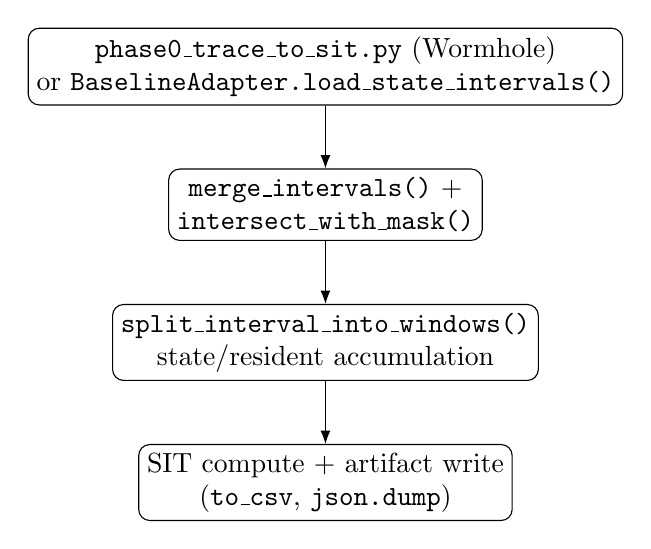
\begin{tikzpicture}[node distance=8mm and 12mm]
\node[box] (a) {\texttt{phase0\_trace\_to\_sit.py} (Wormhole)\\or \texttt{BaselineAdapter.load\_state\_intervals()}};
\node[box, below=of a] (b) {\texttt{merge\_intervals()} +\\\texttt{intersect\_with\_mask()}};
\node[box, below=of b] (c) {\texttt{split\_interval\_into\_windows()}\\state/resident accumulation};
\node[box, below=of c] (d) {SIT compute + artifact write\\(\texttt{to\_csv}, \texttt{json.dump})};
\draw[line] (a) -- (b);
\draw[line] (b) -- (c);
\draw[line] (c) -- (d);
\end{tikzpicture}
\caption{SIT Engine Core Function Flow}
\end{figure}

\end{document}
